\section{Tiefensuche}
\label{sect:tiefensuche}

\begin{bem}
Typische Fragen auf Graphen, deren algorithmische Behandlung grundlegend für viele Anwendungen ist, sind zum Beispiel die folgenden:
\begin{itemize}
 \item Ist der Graph zusammenhängend?
 \item Gibt es einen Pfad im Graphen von einem Knoten $s$ zu einem Knoten $z$?
 \item Wieviele Zusammenhangskomponenten hat der Graph?
 \item Gibt es Kreise oder Zyklen im Graphen?
 \item Was ist der Grad eines gegebenen Knotens?
\end{itemize}

Ein allgemeines Prinzip um diese Art Fragen zu beantworten ist die sogenannte \emph{Graphendurchmusterung}, deren Ziel es ist alle Knoten und Kanten des gegebenen Graphen zu \glqq erkunden\grqq\ und dabei nützliche Informationen über den Graphen zu sammeln.
Die Arbeitsweise und die Effizienz der jeweiligen Algorithmen zur Graphendurchmusterung hängen natürlich stark von der Wahl der Darstellung (Kantenliste, Adjazenzliste, Adjazenzmatrix, Inzidenzmatrix) des Graphen ab.

\end{bem} 

\begin{bem} 
In diesem Abschnitt lernen wir die Durchmusterungsmethode der \emph{Tiefensuche} kennen, die im Englischen \emph{depth first search} heißt und daher oft \emph{DFS} genannt wird.

Die Eingabe für die hier diskutierte Tiefensuche ist ein Digraph $D=(V,A)$.
Ist der Graph ungerichtet, so ist die Vorgehensweise vollkommen analog und daher diskutieren wir hier (fast ausschließlich) die gerichtete Variante.
Der Digraph $D$ ist durch seine Adjazenzliste $N$ gegeben, das heißt, für jeden Knoten $u \in V$ ist $N[u]$ eine Liste aller $v \in V$ mit $(u,v) \in A$.
Wir werden sehen, dass die Darstellung von $D$ als Adjazenzliste eine Durchmusterung mit der optimalen Laufzeit $\Theta(|V|+|A|)$ erlaubt.
\end{bem}

\begin{bem} 
Die Strategie der Tiefensuche besteht darin, einen Startknoten auszuwählen und von diesem ausgehend den Graphen \glqq der Tiefe nach\grqq\ zu durchsuchen.
Das heißt, es werden stets Kanten untersucht, die von dem zuletzt entdeckten Knoten ausgehen, der noch keine bereits untersuchten ausgehenden Kanten hat.
Sobald alle ausgehenden Kanten eines Knotens~$v$ untersucht wurden, geht das Vorgehen einen Schritt zurück und untersucht die Kanten, die von dem Knoten ausgehen, von dem aus~$v$ entdeckt wurde.

Die Umsetzung dieser Strategie basiert auf Farbattributen der Knoten (weiß, grau, schwarz), die im Laufe der Durchmusterung geeignet verändert werden.
Am Anfang des Verfahrens ist jeder Knoten weiß und wenn die Suche entlang einer Kante verläuft, die in einen weißen Knoten endet, dann sagen wir, dass der entsprechende Knoten \emph{entdeckt} wird.

Die Farben der Knoten haben die folgende Bedeutung: 
\begin{itemize}
\setlength{\itemindent}{30pt}
	\item[{\bfseries weiß:}] Der Knoten wurde noch nicht entdeckt. 
	\item[{\bfseries grau:}] Der Knoten wurde entdeckt und die Tiefensuche für den Knoten läuft gerade.
	\item[{\bfseries schwarz:}] Der Knoten wurde entdeckt und die Tiefensuche für den Knoten ist bereits beendet.
\end{itemize}

Wird ein Knoten schwarz gefärbt, so sagen wir auch das er \emph{abgearbeitet} wurde.
\end{bem}

\begin{bem}
Algorithmen zur Tiefensuche -- bzw.~zur Graphendurchmusterung im Allgemeinen -- sammeln zusätzlich nützliche Informationen über die Struktur und die Zusammenhänge im Eingabegraphen auf.
Die Variante der Tiefensuche, die wir hier untersuchen, sammelt Daten in Form der Vorgängerabbildung und den Zeitstempeln:
%
\begin{itemize}
 \item Die \emph{Vorgängerabbildung} ist ein Array~$\pi$ mit $|V|$ Komponenten.
 Durch $\pi[v]$ wird notiert von welchem Knoten aus der Knoten $v$ entdeckt wurde.
 Zum Beginn der Tiefensuche setzt man $\pi[v]=\cc{nil}$ für alle Knoten $v \in V$.

 Die Vorgängerabbildung ermöglicht es zum Beispiel, ausgehend von einem Knoten $s \in V$, für alle erreichbaren Knoten $v \in V$ auch einen $(s,v)$-Pfad auszurechnen.
Setzt man $\pi[v]:=u$ so heißt das, dass jeder $(s,u)$-Pfad $(v_0,\ldots,v_k)$ zu einem $(s,v)$-Pfad $(v_0,\ldots,v_k,v)$ erweitert werden kann.
 \item Jeder Knoten $v \in V$ wird während der Tiefensuche mit zwei \emph{Zeitstempeln} versehen: Der erste Zeitstempel $\cc{Grau}[v]$ zeichnet auf, wann der Knoten grau gefärbt wird, das heißt, wann er das erste Mal entdeckt wird.
Der zweite Zeitstempel $\cc{Schwarz}[v]$ hingegen, speichert den Zeitpunkt der Schwarzfärbung von~$v$, das heißt, den Moment in dem der Knoten abgearbeitet ist.

Im Algorithmus werden beide Zeitstempel ganze Zahlen zwischen $1$ und $2 |V|$ sein, da es für jeden Knoten $v \in V$ genau einen Zeitpunkt der Entdeckung (Graufärbung) und einen Zeitpunkt der Abarbeitung (Schwarzfärbung) gibt.

Für jedes $v \in V$ gilt $\cc{Grau}[v] < \cc{Schwarz}[v]$.
Weiterhin ist $v$ vor dem Zeitpunkt $\cc{Grau}[v]$ weiß, während der Zeitpunkte $\cc{Grau}[v],\ldots,\cc{Schwarz}[v]-1$ grau, und ab dem Zeitpunkt $\cc{Schwarz}[v]$ schwarz.

\end{itemize}
\end{bem}

\begin{bem} 
Nach diesen Vorbereitungen können wir nun die oben bereits diskutierte Vorgehensweise der Tiefensuche algorithmisch exakt umsetzen.


\begin{algorithm}[H]
	\caption{$\cc{Vollständige-Tiefensuche}(D)$}
	\begin{algorithmic}[1]
		\FOR{$u \in V$}
		 \STATE $\cc{Farbe}[u]=\cc{weiß}$
		 \STATE $\pi[u]=\cc{nil}$
		\ENDFOR
		\STATE $t := 0$ $\quad$ \COMMENT{Globale Variable für das Zeitstempeln}
		\FOR{$u \in V$}\label{line:tiefensuche-hauptschleife-start}
 		 \IF{$\cc{Farbe}[u]=\cc{weiß}$}
 		  \STATE $\cc{Tiefensuche}(u)$
 		 \ENDIF 
		\ENDFOR\label{line:tiefensuche-hauptschleife-ende}
	\end{algorithmic}
\end{algorithm}
\end{bem}

\begin{bem} 
Die Prozedur $\cc{Tiefensuche}(u)$ ändert die Farbe des weißen Knotens~$u$ zu grau und \emph{sondiert} anschließend alle Kanten im Graphen, die $u$ als Startknoten haben.
Für den entsprechenden Endknoten $v$ wird die Tiefensuche dann rekursiv aufgerufen.
Sind alle Kanten, die von $u$ ausgehen sondiert, so ist der Knoten~$u$ abgearbeitet und wird schwarz gefärbt.

\begin{algorithm}[H]
	\caption{$\cc{Tiefensuche}(u)$}
	\begin{algorithmic}[1]
		\STATE $t := t + 1$ 
		\STATE $\cc{Grau}[u] := t$ $\quad$ \COMMENT{Der Knoten $u$ wurde gerade entdeckt}
		\STATE $\cc{Farbe}[u]:=\cc{grau}$
		\FOR{$v \in N[u]$}
		\IF{$\cc{Farbe}[v]=\cc{weiß}$}
		 \STATE $\pi[v]:=u$ $\qquad\qquad$ \COMMENT{Die Kante $(u,v)$ wird sondiert}
		\STATE $\cc{Tiefensuche}(v)$
		\ENDIF
		\ENDFOR
		\STATE $t := t + 1$ 
		\STATE\label{line:schwarzfaerbung-in-tiefensuche} $\cc{Schwarz}[u] := t$ $\quad$ \COMMENT{Der Knoten $u$ wurde gerade abgearbeitet}
		\STATE $\cc{Farbe}[u]:=\cc{schwarz}$
	\end{algorithmic}
\end{algorithm}
\end{bem}

\begin{bsp}
\label{bsp:tiefensuche}
Wir illustrieren die Tiefensuche am Digraphen

\hfill
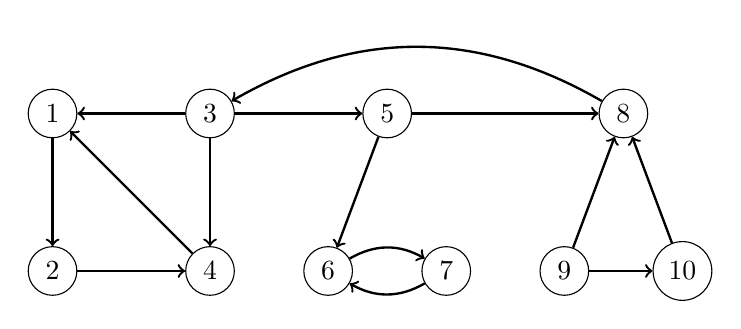
\begin{tikzpicture}[]
 \node[circle,draw=black] (1) at (0,2) {$1$};
 \node[circle,draw=black] (2) at (0,0) {$2$};
 \node[circle,draw=black] (3) at (2,2) {$3$};
 \node[circle,draw=black] (4) at (2,0) {$4$};
 \node[circle,draw=black] (5) at (4.25,2) {$5$};
 \node[circle,draw=black] (6) at (3.5,0) {$6$};
 \node[circle,draw=black] (7) at (5,0) {$7$};
 \node[circle,draw=black] (8) at (7.25,2) {$8$};
 \node[circle,draw=black] (9) at (6.5,0) {$9$};
 \node[circle,draw=black] (10) at (8,0) {$10$};
		
 \draw[->,line width=0.3mm] (1) edge (2);
 \draw[->,line width=0.3mm] (2) edge (4);
 \draw[->,line width=0.3mm] (3) edge (1) (3) edge (4) (3) edge (5);
 \draw[->,line width=0.3mm] (4) edge (1);
 \draw[->,line width=0.3mm] (5) edge (6) (5) edge (8); 
 \draw[->,line width=0.3mm] (6) to[bend left] (7);
 \draw[->,line width=0.3mm] (7) to[bend left] (6);
 \draw[->,line width=0.3mm] (8) to[bend right] (3);
 \draw[->,line width=0.3mm] (9) edge (8) (9) edge (10);
 \draw[->,line width=0.3mm] (10) edge (8); 
\end{tikzpicture}
\hfill\,

Wir wählen als Startknoten den Knoten~$3$ und treffen ansonsten jede Wahl aufsteigend in der Reihenfolge der Knotenindizes.
Die ersten sechs Zeitschritte sind durch die folgende Sequenz von gefärbten Digraphen gegeben, wobei die Knotenfarbe dem aktuellen Farbattribut entspricht und die bereits sondierten Kanten rot markiert sind:

\hfill
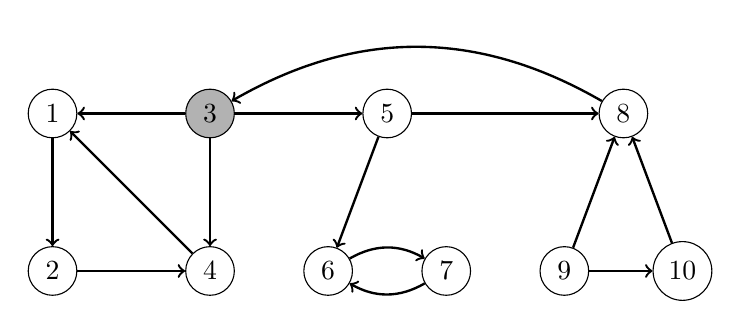
\begin{tikzpicture}[]
 \tikzset{gnode/.style ={fill=black!30!,circle,draw}}
 \tikzset{snode/.style ={fill=black!70!,circle,draw}}

 \node[circle,draw=black] (1) at (0,2) {$1$};
 \node[circle,draw=black] (2) at (0,0) {$2$};
 \node[gnode] (3) at (2,2) {$3$};
 \node[circle,draw=black] (4) at (2,0) {$4$};
 \node[circle,draw=black] (5) at (4.25,2) {$5$};
 \node[circle,draw=black] (6) at (3.5,0) {$6$};
 \node[circle,draw=black] (7) at (5,0) {$7$};
 \node[circle,draw=black] (8) at (7.25,2) {$8$};
 \node[circle,draw=black] (9) at (6.5,0) {$9$};
 \node[circle,draw=black] (10) at (8,0) {$10$};
		
 \draw[->,line width=0.3mm] (1) edge (2);
 \draw[->,line width=0.3mm] (2) edge (4);
 \draw[->,line width=0.3mm] (3) edge (1) (3) edge (4) (3) edge (5);
 \draw[->,line width=0.3mm] (4) edge (1);
 \draw[->,line width=0.3mm] (5) edge (6) (5) edge (8); 
 \draw[->,line width=0.3mm] (6) to[bend left] (7);
 \draw[->,line width=0.3mm] (7) to[bend left] (6);
 \draw[->,line width=0.3mm] (8) to[bend right] (3);
 \draw[->,line width=0.3mm] (9) edge (8) (9) edge (10);
 \draw[->,line width=0.3mm] (10) edge (8); 
\end{tikzpicture}
\hfill\,

\hfill
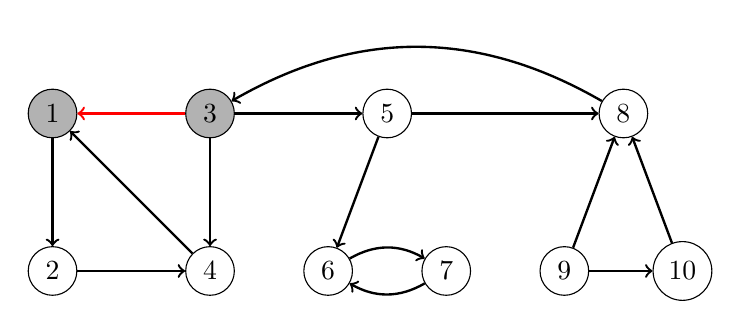
\begin{tikzpicture}[]
 \tikzset{gnode/.style ={fill=black!30!,circle,draw}}
 \tikzset{snode/.style ={fill=black!70!,circle,draw}}

 \node[gnode] (1) at (0,2) {$1$};
 \node[circle,draw=black] (2) at (0,0) {$2$};
 \node[gnode] (3) at (2,2) {$3$};
 \node[circle,draw=black] (4) at (2,0) {$4$};
 \node[circle,draw=black] (5) at (4.25,2) {$5$};
 \node[circle,draw=black] (6) at (3.5,0) {$6$};
 \node[circle,draw=black] (7) at (5,0) {$7$};
 \node[circle,draw=black] (8) at (7.25,2) {$8$};
 \node[circle,draw=black] (9) at (6.5,0) {$9$};
 \node[circle,draw=black] (10) at (8,0) {$10$};
		
 \draw[->,line width=0.3mm] (1) edge (2);
 \draw[->,line width=0.3mm] (2) edge (4);
 \draw[->,line width=0.3mm,red] (3) edge (1);
 \draw[->,line width=0.3mm] (3) edge (4) (3) edge (5);
 \draw[->,line width=0.3mm] (4) edge (1);
 \draw[->,line width=0.3mm] (5) edge (6) (5) edge (8); 
 \draw[->,line width=0.3mm] (6) to[bend left] (7);
 \draw[->,line width=0.3mm] (7) to[bend left] (6);
 \draw[->,line width=0.3mm] (8) to[bend right] (3);
 \draw[->,line width=0.3mm] (9) edge (8) (9) edge (10);
 \draw[->,line width=0.3mm] (10) edge (8); 
\end{tikzpicture}
\hfill\,

\hfill
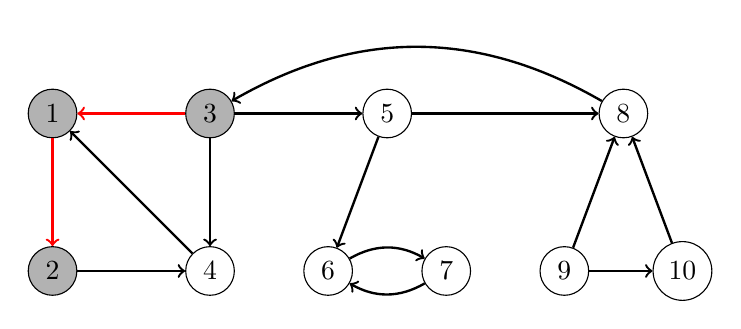
\begin{tikzpicture}[]
 \tikzset{gnode/.style ={fill=black!30!,circle,draw}}
 \tikzset{snode/.style ={fill=black!70!,circle,draw}}

 \node[gnode] (1) at (0,2) {$1$};
 \node[gnode] (2) at (0,0) {$2$};
 \node[gnode] (3) at (2,2) {$3$};
 \node[circle,draw=black] (4) at (2,0) {$4$};
 \node[circle,draw=black] (5) at (4.25,2) {$5$};
 \node[circle,draw=black] (6) at (3.5,0) {$6$};
 \node[circle,draw=black] (7) at (5,0) {$7$};
 \node[circle,draw=black] (8) at (7.25,2) {$8$};
 \node[circle,draw=black] (9) at (6.5,0) {$9$};
 \node[circle,draw=black] (10) at (8,0) {$10$};
		
 \draw[->,line width=0.3mm,red] (1) edge (2);
 \draw[->,line width=0.3mm] (2) edge (4);
 \draw[->,line width=0.3mm,red] (3) edge (1);
 \draw[->,line width=0.3mm] (3) edge (4) (3) edge (5);
 \draw[->,line width=0.3mm] (4) edge (1);
 \draw[->,line width=0.3mm] (5) edge (6) (5) edge (8); 
 \draw[->,line width=0.3mm] (6) to[bend left] (7);
 \draw[->,line width=0.3mm] (7) to[bend left] (6);
 \draw[->,line width=0.3mm] (8) to[bend right] (3);
 \draw[->,line width=0.3mm] (9) edge (8) (9) edge (10);
 \draw[->,line width=0.3mm] (10) edge (8); 
\end{tikzpicture}
\hfill\,

\hfill
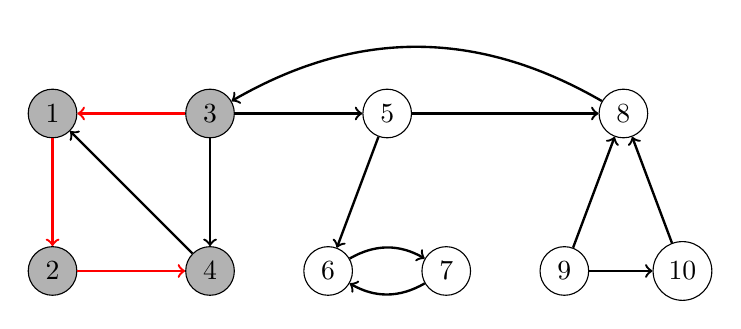
\begin{tikzpicture}[]
 \tikzset{gnode/.style ={fill=black!30!,circle,draw}}
 \tikzset{snode/.style ={fill=black!70!,circle,draw}}

 \node[gnode] (1) at (0,2) {$1$};
 \node[gnode] (2) at (0,0) {$2$};
 \node[gnode] (3) at (2,2) {$3$};
 \node[gnode] (4) at (2,0) {$4$};
 \node[circle,draw=black] (5) at (4.25,2) {$5$};
 \node[circle,draw=black] (6) at (3.5,0) {$6$};
 \node[circle,draw=black] (7) at (5,0) {$7$};
 \node[circle,draw=black] (8) at (7.25,2) {$8$};
 \node[circle,draw=black] (9) at (6.5,0) {$9$};
 \node[circle,draw=black] (10) at (8,0) {$10$};
		
 \draw[->,line width=0.3mm,red] (1) edge (2);
 \draw[->,line width=0.3mm,red] (2) edge (4);
 \draw[->,line width=0.3mm,red] (3) edge (1);
 \draw[->,line width=0.3mm] (3) edge (4) (3) edge (5);
 \draw[->,line width=0.3mm] (4) edge (1);
 \draw[->,line width=0.3mm] (5) edge (6) (5) edge (8); 
 \draw[->,line width=0.3mm] (6) to[bend left] (7);
 \draw[->,line width=0.3mm] (7) to[bend left] (6);
 \draw[->,line width=0.3mm] (8) to[bend right] (3);
 \draw[->,line width=0.3mm] (9) edge (8) (9) edge (10);
 \draw[->,line width=0.3mm] (10) edge (8); 
\end{tikzpicture}
\hfill\,

\hfill
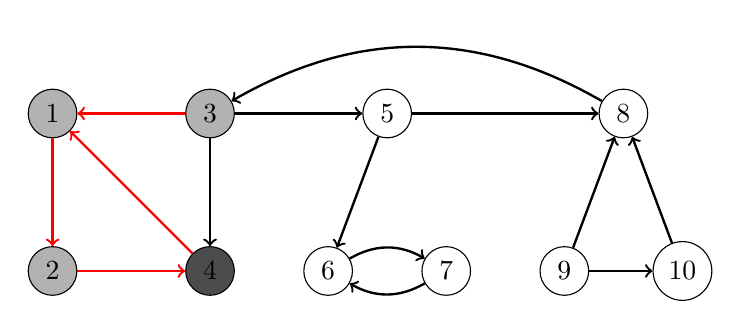
\begin{tikzpicture}[]
 \tikzset{gnode/.style ={fill=black!30!,circle,draw}}
 \tikzset{snode/.style ={fill=black!70!,circle,draw}}

 \node[gnode] (1) at (0,2) {$1$};
 \node[gnode] (2) at (0,0) {$2$};
 \node[gnode] (3) at (2,2) {$3$};
 \node[snode] (4) at (2,0) {$4$};
 \node[circle,draw=black] (5) at (4.25,2) {$5$};
 \node[circle,draw=black] (6) at (3.5,0) {$6$};
 \node[circle,draw=black] (7) at (5,0) {$7$};
 \node[circle,draw=black] (8) at (7.25,2) {$8$};
 \node[circle,draw=black] (9) at (6.5,0) {$9$};
 \node[circle,draw=black] (10) at (8,0) {$10$};
		
 \draw[->,line width=0.3mm,red] (1) edge (2);
 \draw[->,line width=0.3mm,red] (2) edge (4);
 \draw[->,line width=0.3mm,red] (3) edge (1);
 \draw[->,line width=0.3mm] (3) edge (4) (3) edge (5);
 \draw[->,line width=0.3mm,red] (4) edge (1);
 \draw[->,line width=0.3mm] (5) edge (6) (5) edge (8); 
 \draw[->,line width=0.3mm] (6) to[bend left] (7);
 \draw[->,line width=0.3mm] (7) to[bend left] (6);
 \draw[->,line width=0.3mm] (8) to[bend right] (3);
 \draw[->,line width=0.3mm] (9) edge (8) (9) edge (10);
 \draw[->,line width=0.3mm] (10) edge (8); 
\end{tikzpicture}
\hfill\,

\hfill
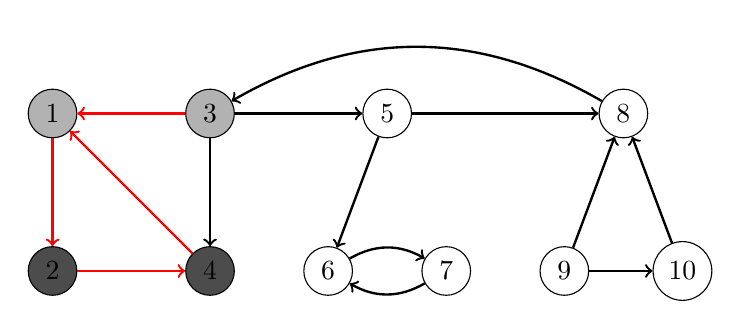
\begin{tikzpicture}[]
 \tikzset{gnode/.style ={fill=black!30!,circle,draw}}
 \tikzset{snode/.style ={fill=black!70!,circle,draw}}

 \node[gnode] (1) at (0,2) {$1$};
 \node[snode] (2) at (0,0) {$2$};
 \node[gnode] (3) at (2,2) {$3$};
 \node[snode] (4) at (2,0) {$4$};
 \node[circle,draw=black] (5) at (4.25,2) {$5$};
 \node[circle,draw=black] (6) at (3.5,0) {$6$};
 \node[circle,draw=black] (7) at (5,0) {$7$};
 \node[circle,draw=black] (8) at (7.25,2) {$8$};
 \node[circle,draw=black] (9) at (6.5,0) {$9$};
 \node[circle,draw=black] (10) at (8,0) {$10$};
		
 \draw[->,line width=0.3mm,red] (1) edge (2);
 \draw[->,line width=0.3mm,red] (2) edge (4);
 \draw[->,line width=0.3mm,red] (3) edge (1);
 \draw[->,line width=0.3mm] (3) edge (4) (3) edge (5);
 \draw[->,line width=0.3mm,red] (4) edge (1);
 \draw[->,line width=0.3mm] (5) edge (6) (5) edge (8); 
 \draw[->,line width=0.3mm] (6) to[bend left] (7);
 \draw[->,line width=0.3mm] (7) to[bend left] (6);
 \draw[->,line width=0.3mm] (8) to[bend right] (3);
 \draw[->,line width=0.3mm] (9) edge (8) (9) edge (10);
 \draw[->,line width=0.3mm] (10) edge (8); 
\end{tikzpicture}
\hfill\,

Wir steigen zum Zeitpunkt $\cc{Schwarz}[8]=14$ mit der Illustration wieder ein:

\hfill
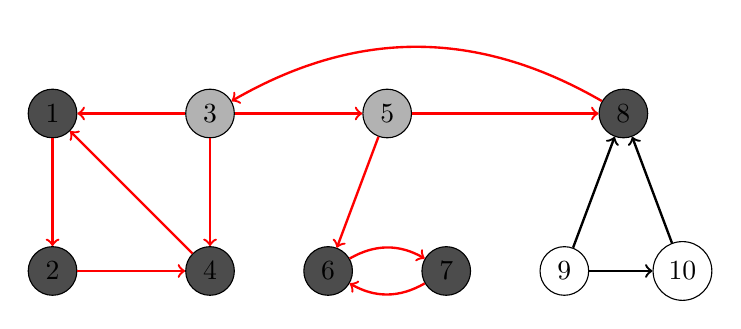
\begin{tikzpicture}[]
 \tikzset{gnode/.style ={fill=black!30!,circle,draw}}
 \tikzset{snode/.style ={fill=black!70!,circle,draw}}

 \node[snode] (1) at (0,2) {$1$};
 \node[snode] (2) at (0,0) {$2$};
 \node[gnode] (3) at (2,2) {$3$};
 \node[snode] (4) at (2,0) {$4$};
 \node[gnode] (5) at (4.25,2) {$5$};
 \node[snode] (6) at (3.5,0) {$6$};
 \node[snode] (7) at (5,0) {$7$};
 \node[snode] (8) at (7.25,2) {$8$};
 \node[circle,draw=black] (9) at (6.5,0) {$9$};
 \node[circle,draw=black] (10) at (8,0) {$10$};
		
 \draw[->,line width=0.3mm,red] (1) edge (2);
 \draw[->,line width=0.3mm,red] (2) edge (4);
 \draw[->,line width=0.3mm,red] (3) edge (1);
 \draw[->,line width=0.3mm,red] (3) edge (4) (3) edge (5);
 \draw[->,line width=0.3mm,red] (4) edge (1);
 \draw[->,line width=0.3mm,red] (5) edge (6) (5) edge (8); 
 \draw[->,line width=0.3mm,red] (6) to[bend left] (7);
 \draw[->,line width=0.3mm,red] (7) to[bend left] (6);
 \draw[->,line width=0.3mm,red] (8) to[bend right] (3);
 \draw[->,line width=0.3mm] (9) edge (8) (9) edge (10);
 \draw[->,line width=0.3mm] (10) edge (8); 
\end{tikzpicture}
\hfill\,

\hfill
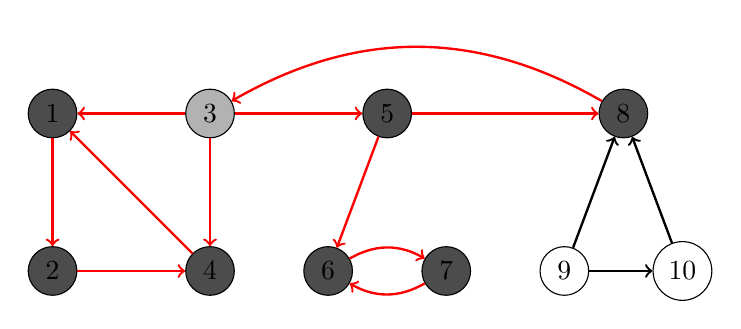
\begin{tikzpicture}[]
 \tikzset{gnode/.style ={fill=black!30!,circle,draw}}
 \tikzset{snode/.style ={fill=black!70!,circle,draw}}

 \node[snode] (1) at (0,2) {$1$};
 \node[snode] (2) at (0,0) {$2$};
 \node[gnode] (3) at (2,2) {$3$};
 \node[snode] (4) at (2,0) {$4$};
 \node[snode] (5) at (4.25,2) {$5$};
 \node[snode] (6) at (3.5,0) {$6$};
 \node[snode] (7) at (5,0) {$7$};
 \node[snode] (8) at (7.25,2) {$8$};
 \node[circle,draw=black] (9) at (6.5,0) {$9$};
 \node[circle,draw=black] (10) at (8,0) {$10$};
		
 \draw[->,line width=0.3mm,red] (1) edge (2);
 \draw[->,line width=0.3mm,red] (2) edge (4);
 \draw[->,line width=0.3mm,red] (3) edge (1);
 \draw[->,line width=0.3mm,red] (3) edge (4) (3) edge (5);
 \draw[->,line width=0.3mm,red] (4) edge (1);
 \draw[->,line width=0.3mm,red] (5) edge (6) (5) edge (8); 
 \draw[->,line width=0.3mm,red] (6) to[bend left] (7);
 \draw[->,line width=0.3mm,red] (7) to[bend left] (6);
 \draw[->,line width=0.3mm,red] (8) to[bend right] (3);
 \draw[->,line width=0.3mm] (9) edge (8) (9) edge (10);
 \draw[->,line width=0.3mm] (10) edge (8); 
\end{tikzpicture}
\hfill\,

\hfill
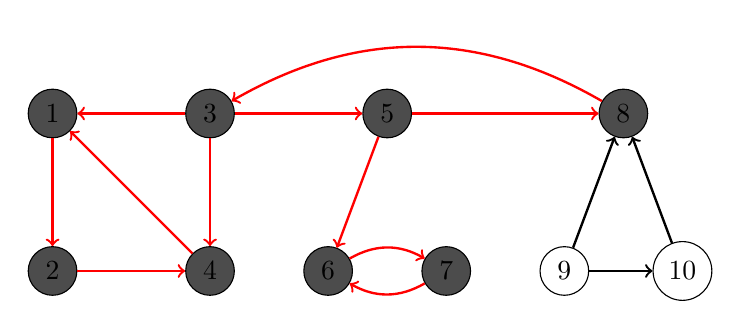
\begin{tikzpicture}[]
 \tikzset{gnode/.style ={fill=black!30!,circle,draw}}
 \tikzset{snode/.style ={fill=black!70!,circle,draw}}

 \node[snode] (1) at (0,2) {$1$};
 \node[snode] (2) at (0,0) {$2$};
 \node[snode] (3) at (2,2) {$3$};
 \node[snode] (4) at (2,0) {$4$};
 \node[snode] (5) at (4.25,2) {$5$};
 \node[snode] (6) at (3.5,0) {$6$};
 \node[snode] (7) at (5,0) {$7$};
 \node[snode] (8) at (7.25,2) {$8$};
 \node[circle,draw=black] (9) at (6.5,0) {$9$};
 \node[circle,draw=black] (10) at (8,0) {$10$};
		
 \draw[->,line width=0.3mm,red] (1) edge (2);
 \draw[->,line width=0.3mm,red] (2) edge (4);
 \draw[->,line width=0.3mm,red] (3) edge (1);
 \draw[->,line width=0.3mm,red] (3) edge (4) (3) edge (5);
 \draw[->,line width=0.3mm,red] (4) edge (1);
 \draw[->,line width=0.3mm,red] (5) edge (6) (5) edge (8); 
 \draw[->,line width=0.3mm,red] (6) to[bend left] (7);
 \draw[->,line width=0.3mm,red] (7) to[bend left] (6);
 \draw[->,line width=0.3mm,red] (8) to[bend right] (3);
 \draw[->,line width=0.3mm] (9) edge (8) (9) edge (10);
 \draw[->,line width=0.3mm] (10) edge (8); 
\end{tikzpicture}
\hfill\,

Nun muss ein neuer Knoten gewählt werden (Knoten $9$) um die Tiefensuche für den ganzen Digraphen zu beenden:

\hfill
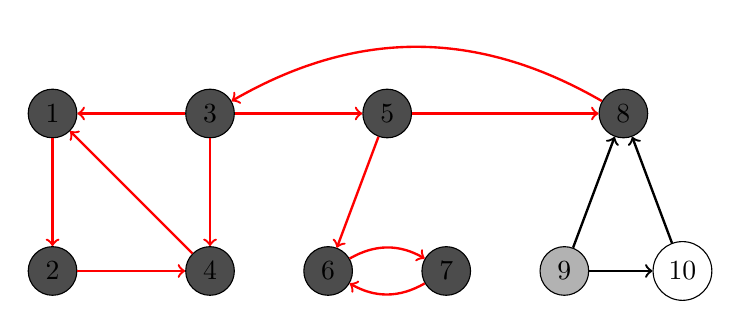
\begin{tikzpicture}[]
 \tikzset{gnode/.style ={fill=black!30!,circle,draw}}
 \tikzset{snode/.style ={fill=black!70!,circle,draw}}

 \node[snode] (1) at (0,2) {$1$};
 \node[snode] (2) at (0,0) {$2$};
 \node[snode] (3) at (2,2) {$3$};
 \node[snode] (4) at (2,0) {$4$};
 \node[snode] (5) at (4.25,2) {$5$};
 \node[snode] (6) at (3.5,0) {$6$};
 \node[snode] (7) at (5,0) {$7$};
 \node[snode] (8) at (7.25,2) {$8$};
 \node[gnode] (9) at (6.5,0) {$9$};
 \node[circle,draw=black] (10) at (8,0) {$10$};
		
 \draw[->,line width=0.3mm,red] (1) edge (2);
 \draw[->,line width=0.3mm,red] (2) edge (4);
 \draw[->,line width=0.3mm,red] (3) edge (1);
 \draw[->,line width=0.3mm,red] (3) edge (4) (3) edge (5);
 \draw[->,line width=0.3mm,red] (4) edge (1);
 \draw[->,line width=0.3mm,red] (5) edge (6) (5) edge (8); 
 \draw[->,line width=0.3mm,red] (6) to[bend left] (7);
 \draw[->,line width=0.3mm,red] (7) to[bend left] (6);
 \draw[->,line width=0.3mm,red] (8) to[bend right] (3);
 \draw[->,line width=0.3mm] (9) edge (8) (9) edge (10);
 \draw[->,line width=0.3mm] (10) edge (8); 
\end{tikzpicture}
\hfill\,

\hfill
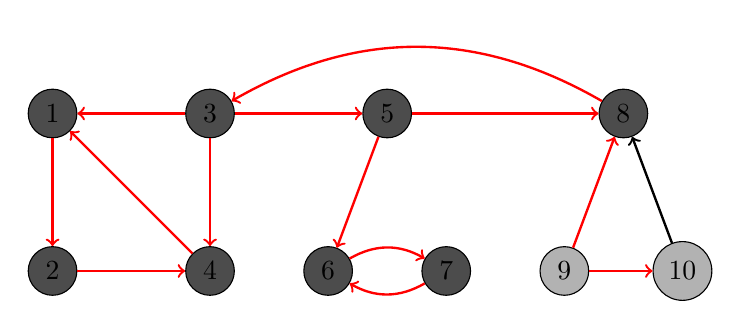
\begin{tikzpicture}[]
 \tikzset{gnode/.style ={fill=black!30!,circle,draw}}
 \tikzset{snode/.style ={fill=black!70!,circle,draw}}

 \node[snode] (1) at (0,2) {$1$};
 \node[snode] (2) at (0,0) {$2$};
 \node[snode] (3) at (2,2) {$3$};
 \node[snode] (4) at (2,0) {$4$};
 \node[snode] (5) at (4.25,2) {$5$};
 \node[snode] (6) at (3.5,0) {$6$};
 \node[snode] (7) at (5,0) {$7$};
 \node[snode] (8) at (7.25,2) {$8$};
 \node[gnode] (9) at (6.5,0) {$9$};
 \node[gnode] (10) at (8,0) {$10$};
		
 \draw[->,line width=0.3mm,red] (1) edge (2);
 \draw[->,line width=0.3mm,red] (2) edge (4);
 \draw[->,line width=0.3mm,red] (3) edge (1);
 \draw[->,line width=0.3mm,red] (3) edge (4) (3) edge (5);
 \draw[->,line width=0.3mm,red] (4) edge (1);
 \draw[->,line width=0.3mm,red] (5) edge (6) (5) edge (8); 
 \draw[->,line width=0.3mm,red] (6) to[bend left] (7);
 \draw[->,line width=0.3mm,red] (7) to[bend left] (6);
 \draw[->,line width=0.3mm,red] (8) to[bend right] (3);
 \draw[->,line width=0.3mm,red] (9) edge (8) (9) edge (10);
 \draw[->,line width=0.3mm] (10) edge (8); 
\end{tikzpicture}
\hfill\,

\hfill
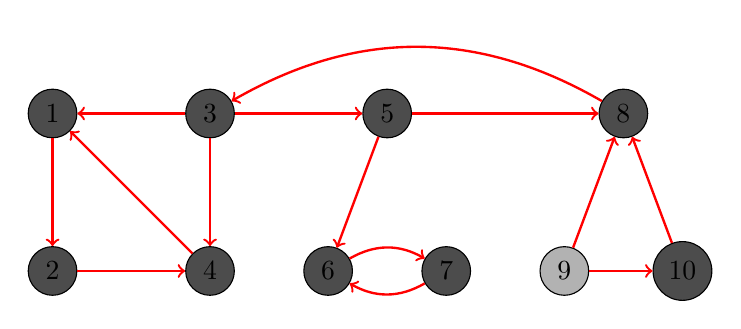
\begin{tikzpicture}[]
 \tikzset{gnode/.style ={fill=black!30!,circle,draw}}
 \tikzset{snode/.style ={fill=black!70!,circle,draw}}

 \node[snode] (1) at (0,2) {$1$};
 \node[snode] (2) at (0,0) {$2$};
 \node[snode] (3) at (2,2) {$3$};
 \node[snode] (4) at (2,0) {$4$};
 \node[snode] (5) at (4.25,2) {$5$};
 \node[snode] (6) at (3.5,0) {$6$};
 \node[snode] (7) at (5,0) {$7$};
 \node[snode] (8) at (7.25,2) {$8$};
 \node[gnode] (9) at (6.5,0) {$9$};
 \node[snode] (10) at (8,0) {$10$};
		
 \draw[->,line width=0.3mm,red] (1) edge (2);
 \draw[->,line width=0.3mm,red] (2) edge (4);
 \draw[->,line width=0.3mm,red] (3) edge (1);
 \draw[->,line width=0.3mm,red] (3) edge (4) (3) edge (5);
 \draw[->,line width=0.3mm,red] (4) edge (1);
 \draw[->,line width=0.3mm,red] (5) edge (6) (5) edge (8); 
 \draw[->,line width=0.3mm,red] (6) to[bend left] (7);
 \draw[->,line width=0.3mm,red] (7) to[bend left] (6);
 \draw[->,line width=0.3mm,red] (8) to[bend right] (3);
 \draw[->,line width=0.3mm,red] (9) edge (8) (9) edge (10);
 \draw[->,line width=0.3mm,red] (10) edge (8); 
\end{tikzpicture}
\hfill\,

\hfill
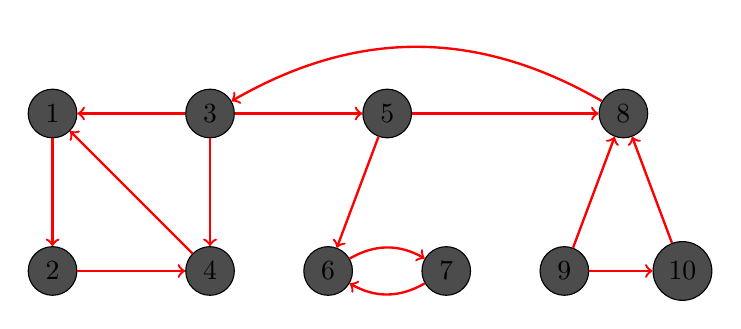
\begin{tikzpicture}[]
 \tikzset{gnode/.style ={fill=black!30!,circle,draw}}
 \tikzset{snode/.style ={fill=black!70!,circle,draw}}

 \node[snode] (1) at (0,2) {$1$};
 \node[snode] (2) at (0,0) {$2$};
 \node[snode] (3) at (2,2) {$3$};
 \node[snode] (4) at (2,0) {$4$};
 \node[snode] (5) at (4.25,2) {$5$};
 \node[snode] (6) at (3.5,0) {$6$};
 \node[snode] (7) at (5,0) {$7$};
 \node[snode] (8) at (7.25,2) {$8$};
 \node[snode] (9) at (6.5,0) {$9$};
 \node[snode] (10) at (8,0) {$10$};
		
 \draw[->,line width=0.3mm,red] (1) edge (2);
 \draw[->,line width=0.3mm,red] (2) edge (4);
 \draw[->,line width=0.3mm,red] (3) edge (1);
 \draw[->,line width=0.3mm,red] (3) edge (4) (3) edge (5);
 \draw[->,line width=0.3mm,red] (4) edge (1);
 \draw[->,line width=0.3mm,red] (5) edge (6) (5) edge (8); 
 \draw[->,line width=0.3mm,red] (6) to[bend left] (7);
 \draw[->,line width=0.3mm,red] (7) to[bend left] (6);
 \draw[->,line width=0.3mm,red] (8) to[bend right] (3);
 \draw[->,line width=0.3mm,red] (9) edge (8) (9) edge (10);
 \draw[->,line width=0.3mm,red] (10) edge (8); 
\end{tikzpicture}
\hfill\,

Nun sind alle Knoten schwarz und die Tiefensuche ist beendet.
\end{bsp}

%Als Beispiel kann man die TS mit dem Startknoten $1$ im Fall von $N$:
%\[
%	\begin{array}{llll}
%	1: & 2, & 4 
%	\\ 2: & 3
%	\\ 3: & 
%	\\ 4: & 2, & 3, & 5
%	\\ 5: & 6
%	\\ 6: & 4
%	\\ 7: & 6
%	\end{array}
%\]
%betrachten. Wir protokollieren die Änderungen wann welche TSen aufgerufen und beendet werden und wie sich die Farben der Knoten ändern. *****

Wir überzeugen uns nun davon, dass die oben beschriebene Tiefensuche die angekündigte Laufzeit hat, wenn der Eingabedigraph als Adjazenzliste dargestellt ist.

\begin{thm}
\label{thm:laufzeit-tiefensuche}
Es sei ein Digraph $D=(V,A)$ durch eine Adjazenzliste gegeben.
Die Laufzeit von $\cc{Vollständige-Tiefensuche}(D)$ ist $\Theta(|V|+|A|)$.
\end{thm}

\begin{proof}
Nach der Initialisierung der Arrays $\cc{Farbe}$ und $\pi$, die jeweils $\Theta(|V|)$ Zeiteinheiten benötigen, werden die folgende Operationen ausgeführt: Änderung der Farben, Aufruf von $\cc{Tiefensuche}(u)$ für unterschiedliche Knoten $u$, sowie Sondierung der Kanten.
Jeder entdeckte Knoten ändert seine Farbe von weiß zu grau und anschließend zu schwarz.
Da eine Tiefensuche nur für einen weißen Knoten gestartet wird, wird $\cc{Tiefensuche}(u)$ für jeden Knoten~$u$ höchstens ein Mal ausgeführt.
Somit dauert die Bearbeitung von jedem Knoten (Farbenänderung, Aufruf der Tiefensuche) $\Theta(1)$ Zeiteinheiten.
Eine Kante $(u,v) \in A$ kann nur dann sondiert werden, wenn die Tiefensuche für $u$ aufgerufen wird.
Somit kann jede Kante höchstens ein Mal sondiert werden.
Das Sondieren jeder Kante benötigt dadurch $\Theta(1)$ Zeiteinheiten.
Der Gesamtaufwand von $\cc{Vollständige-Tiefensuche}(D)$ ist somit $\Theta(|V|+|A|)$. 
\end{proof}


%\begin{thm}
%	Sei $G=(V,E)$ Digraph mit $m \in \N$ Kanten und $n \in \N$ Knoten, der durch eine Adjazenzliste gegeben ist. Sei $s \in V$. Dan gilt für die Tiefensuche auf $G$ mit dem Startknoten $s$:
%	\begin{enumerate}[(a)]
%		\item Die Laufzeit des Verfahrens ist $O(m+n)$ (das heißt, höchstens $c(m+n)$ für eine Konstante $c>0$).
%		\item Die Menge aller Knoten von $G$, die von $s$ aus durch einen Pfad erreichbar sind ist genau die Menge der Knoten, die während der Ausführung entdeckt werden. 
%		\item Der Graph $G$ enthält genau dann einen von $s$ aus erreichbaren Zyklus, wenn während der Ausführung beim Sondieren einer der Kanten $(u,v)$ die Farbe von $v$ grau ist. 
%	\end{enumerate} 
%\end{thm}
%\begin{proof}
%	(a): Während der Ausführung werden die folgende Operationen ausgeführt: Änderung der Farben und Aufruf der TS für unterschiedliche Knoten sowie Sondierung der Kanten. Jeder entdeckte Knoten ändert seine Farbe von weiß zu grau und anschließend zu schwarz. Da eine TS nur für einen weißen Knoten gestartet wird, wird die TS für jeden Knoten höchstens ein mal ausgeführt. Somit dauert die Bearbeitung von jedem Knoten (Farbenänderung, Aufruf der TS) $O(1)$ Zeiteinheiten. Eine Kante $(u,v)$ wird genau dann sondiert, wenn die TS für $u$ aufgerufen wird. Somit kann jede Kante höchstens ein mal sondiert werden. Das Sondieren jeder Kante beträgt dadurch höchstens $O(1)$ Zeiteinheiten. Der Gesamtaufwand der TS mit dem Startknoten $s$ ist somit $O(m+n)$. 
%	
%	(b): Seien $u_1,\ldots,u_k$ alle Knoten, die während der Ausführung entdeckt werden und seien $u_1,\ldots,u_k$ in dieser Reihenfolge entdeckt ($u_1$ ist der erste entdeckte Knoten, $u_2$ der zweite usw.). Dann ist $u_1$ von $s$ aus erreichbar, denn $u_1=s$. Die TS für einen Knoten $u_j$ mit $j > 1$ wird aus einer TS für einen Knoten $u_i$ aufgerufen, der im Moment der Aufuruf von $TS(u_j)$ bereits entdeckt ist. Man hat also $j< i$. Wenn $u_j$ von $s$ aus erreichbar ist, so ist auch $u_i$ von $s$ aus erreichbar, da $(u_i,u_j)$ eine Kante von $G$ ist. Somit folgt durch Induktion über $j$, das jeder Knoten $u_j$ von $s$ aus erreichbar ist. 
%	
%	Umgekehrt zeigen wir nun, dass jeder Knoten $v \in V$, der von $s$ aus erreichbar ist, während der Ausführung entdeckt wird. Sei $(v_0,\ldots,v_k)$ ein Pfad von $s$ nach $v$. Wir zeigen nun, dass jeder Knoten $v_j$ dieses Pfades entdeckt wird. Für $v_0=s$ gilt die Aussage offensichtlich. Wird ein Knoten $v_j$ mit $j < k$ entdeckt, so entdeckt man den Knoten $v_{j+1}$ spätestens beim Sondieren der Kante $(v_j,v_{j+1})$ innerhalb der TS für $v_j$. Es kann als durch Induktion über $j$ gezeigt werden, dass alle $v_j$ und insbesondere auch $v_k=v$ entdeckt werden.
%	
%	(c): Der Beweis von (c) ist analog zum Beweis von (b) und wird hier nicht angeführt. (Aufgabe)
%\end{proof}
%

\subsection{Eigenschaften der Tiefensuche}

\begin{defn} 
Die Vorgängerabbildung $\pi$ erzeugt den sogenannten \emph{Vorgängerteilgraphen} eines Digraphen $D=(V,A)$, der formal durch $D_\pi=(V,A_\pi)$ mit
\[
A_\pi = \left\{(\pi[v],v) : v \in V \text{ und } \pi[v] \neq \cc{nil}\right\}
\]
definiert ist.
Für jede Tiefensuche ist der Vorgängerteilgraph ein Wald, und wird daher im Folgenden als \emph{Tiefensuchwald} bezeichnet.
Er ist aus einem oder mehreren \emph{Tiefensuchbäumen} zusammengesetzt.
\end{defn} 

\begin{bsp} 
In Beispiel~\ref{bsp:tiefensuche} ist die Vorgängerabbildung nach abgeschlossener Tiefensuche durch $\pi=[3,1,\cc{nil},2,3,5,6,5,\cc{nil},9]$ gegeben.
Der zugehörige Tiefensuchwald ist also

\hfill
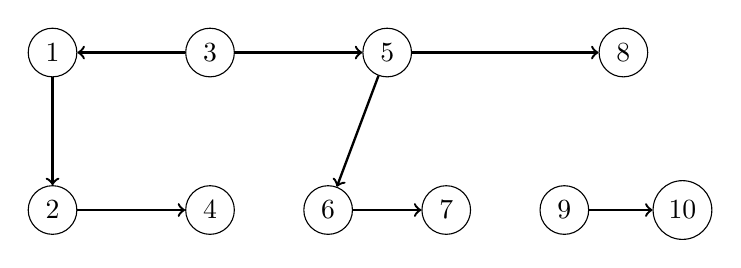
\begin{tikzpicture}[]
 \node[circle,draw=black] (1) at (0,2) {$1$};
 \node[circle,draw=black] (2) at (0,0) {$2$};
 \node[circle,draw=black] (3) at (2,2) {$3$};
 \node[circle,draw=black] (4) at (2,0) {$4$};
 \node[circle,draw=black] (5) at (4.25,2) {$5$};
 \node[circle,draw=black] (6) at (3.5,0) {$6$};
 \node[circle,draw=black] (7) at (5,0) {$7$};
 \node[circle,draw=black] (8) at (7.25,2) {$8$};
 \node[circle,draw=black] (9) at (6.5,0) {$9$};
 \node[circle,draw=black] (10) at (8,0) {$10$};
		
 \draw[->,line width=0.3mm] (1) edge (2);
 \draw[->,line width=0.3mm] (2) edge (4);
 \draw[->,line width=0.3mm] (3) edge (1) (3) edge (5);
 \draw[->,line width=0.3mm] (5) edge (6) (5) edge (8); 
 \draw[->,line width=0.3mm] (6) edge (7);
 \draw[->,line width=0.3mm] (9) edge (10);
\end{tikzpicture}
\end{bsp} 

\begin{bem}
Eine erste wichtige Eigenschaft der Tiefensuche ist der Zusammenhang von Entdeckungszeit und Abarbeitungszeit eines Knotens.
Es stellt sich heraus, dass diese Zeitpunkte im folgenden Sinne eine \emph{Klammerstruktur} aufweisen:
Stellen wir die Entdeckungszeit eines Knotens $u$ durch den Ausdruck \glqq $(u$\grqq\ und die Abarbeitungszeit von~$u$ durch den Ausdruck \glqq $u)$\grqq\ dar, dann ergibt die gesamte Historie, über alle Knoten des (Di)Graphen hinweg gesehen, einen korrekt geklammerten Ausdruck.
\end{bem} 

\begin{bsp} 
Zur Illustration dieses Zusammenhangs sehen wir uns wieder die Tiefensuche aus Beispiel~\ref{bsp:tiefensuche} an.
Die Daten der Zeitstempel sind in folgender Tabelle zusammengefasst:
\begin{table}[H]
\centering
\begin{tabular}{|c|c|c|c|c|c|c|c|c|c|c|}
\hline
\textbf{Knoten $u$}        & \textbf{1} & \textbf{2} & \textbf{3} & \textbf{4} & \textbf{5} & \textbf{6} & \textbf{7} & \textbf{8} & \textbf{9} & \textbf{10} \\ \hline
\textbf{$\cc{Grau}[u]$}    & 2          & 3          & 1          & 4          & 8          & 9          & 10         & 13         & 17         & 18          \\ \hline
\textbf{$\cc{Schwarz}[u]$} & 7          & 6          & 16         & 5          & 15         & 12         & 11         & 14         & 20         & 19          \\ \hline
\end{tabular}
\end{table}
Nach obiger Vorschrift können wir damit den zugehörigen Klammerausdruck
\[
(3\ (1\ (2\ (4\ 4)\ 2)\ 1)\ (5\ (6\ (7\ 7)\ 6)\ (8\ 8)\ 5)\ 3)\ (9\ (10\ 10)\ 9)
\]
ablesen.

Eine andere Möglichkeit diese Klammerstruktur auszudrücken ist im folgenden Satz festgehalten:
\end{bsp} 

\begin{thm}[Klammerungstheorem]
\label{thm:klammerung}
Bei der Tiefensuche auf einem Digraphen $D=(V,A)$ ist für jedes Paar von Knoten $u$ und $v$ genau eine der drei folgenden Bedingungen erfüllt:
\begin{enuma}

 \item Die Intervalle $\left[\cc{Grau}[u],\cc{Schwarz}[u]\right]$ und $[\cc{Grau}[v],\cc{Schwarz}[v]]$ sind disjunkt und weder $u$ noch $v$ ist im Tiefensuchwald ein Nachfahre des anderen.

 \item Das Intervall $\left[\cc{Grau}[u],\cc{Schwarz}[u]\right]$ ist im Intervall $[\cc{Grau}[v],\cc{Schwarz}[v]]$ enthalten und $u$ ist im Tiefensuchwald ein Nachfahre von $v$.

 \item Das Intervall $\left[\cc{Grau}[v],\cc{Schwarz}[v]\right]$ ist im Intervall $[\cc{Grau}[u],\cc{Schwarz}[u]]$ enthalten und $v$ ist im Tiefensuchwald ein Nachfahre von $u$.

\end{enuma}
\end{thm}

\begin{proof}
Betrachten wir zunächst den Fall, dass $\cc{Grau}[u] < \cc{Grau}[v]$ ist.
Wir müssen zwei Teilfälle unterscheiden:

\emph{Teilfall 1} ($\cc{Grau}[v] < \cc{Schwarz}[u]$):
Hier wurde also der Knoten~$v$ entdeckt als~$u$ noch grau war.
Demzufolge ist~$v$ ein Nachfahre von~$u$.
Da~$v$ später als~$u$ entdeckt wurde, sind weiterhin alle aus~$v$ austretenden Kanten sondiert und~$v$ ist abgearbeitet, bevor die Tiefensuche zu~$u$ zurückkehrt und diesen Knoten fertig abarbeitet.
Das Intervall $\left[\cc{Grau}[v],\cc{Schwarz}[v]\right]$ ist damit vollständig im Intervall $[\cc{Grau}[u],\cc{Schwarz}[u]]$ enthalten und wir sind im Fall (c) des Theorems.

\emph{Teilfall 2} ($\cc{Grau}[v] > \cc{Schwarz}[u]$):
Da nach Definition für jeden Knoten $r \in V$ die Ungleichung $\cc{Grau}[r] < \cc{Schwarz}[r]$ gilt, sehen wir sofort, dass die Intervalle $\left[\cc{Grau}[u],\cc{Schwarz}[u]\right]$ und $[\cc{Grau}[v],\cc{Schwarz}[v]]$ disjunkt sind.
Daher wurde auch keiner der beiden Knoten entdeckt, während der andere grau war, was nichts anderes heißt, als dass keiner der beiden Knoten Nachfahre des jeweils anderen ist.
Wir sind also im Fall (a) des Theorems.

Im Falle, dass $\cc{Grau}[u] > \cc{Grau}[v]$ ist, argumentieren wir vollkommen analog zu oben; wir müssen lediglich die Rollen von~$u$ und~$v$ vertauschen.
\end{proof}

\begin{bem}
Als direkte Konsequenz des Klammerungstheorems erhalten wir eine Charakterisierung der Nachfahren im Tiefensuchwald eines gegebenen Knotens.
\end{bem} 

\begin{kor}
\label{cor:nachfahre-tiefenwald}
Der Knoten $v$ ist in einem Tiefensuchwald eines Digraphen genau dann ein echter Nachfahre eines Knotens $u$, wenn
\[
\cc{Grau}[u] < \cc{Grau}[v] < \cc{Schwarz}[v]  < \cc{Schwarz}[u].
\]
\end{kor}

\begin{bem} 
Eine alternative Charakterisierung der Nachfahreneigenschaft in Tiefensuchwäldern, die allerdings über die Farben der Knoten während der Suche geht, wird uns später bei den Anwendungen der Tiefensuche nützlich sein. 
\end{bem} 

\begin{thm}[Theorem der weißen Pfade]
\label{thm:weisse-pfade-thm}
Der Knoten $v$ ist in einem Tiefensuchwald eines Digraphen $D=(V,A)$ genau dann ein Nachfahre eines Knotens $u$, wenn es zum Zeitpunkt $\cc{Grau}[u]$, zu dem die Durchmusterung den Knoten~$u$ entdeckt hat, einen Pfad von $u$ nach $v$ gibt, der, bis auf den Knoten $u$, nur aus weißen Knoten besteht.
\end{thm}

\begin{proof}
\glqq $\Longrightarrow$\grqq: Ist $v=u$, so enthält der Pfad von~$u$ nach~$v$ nur den grauen Knoten~$u$ und die Aussage des Theorems gilt.
Ist $v$ ein echter Nachfahre von~$u$ im Tiefensuchwald, so gilt nach Korollar~\ref{cor:nachfahre-tiefenwald}, dass $\cc{Grau}[u] < \cc{Grau}[v]$.
Der Knoten~$v$ ist somit zum Zeitpunkt $\cc{Grau}[u]$ weiß.
Da~$v$ ein beliebiger Nachfolger von~$u$ ist, sind also alle Knoten auf dem einzigen Weg von $u$ nach $v$ im Tiefensuchwald weiß, mit Ausnahme vom Startknoten~$u$ selbst.

\glqq $\Longleftarrow$\grqq: Zum Zwecke eines Widerspruches nehmen wir an, dass es zum Zeitpunkt $\cc{Grau}[u]$ einen Pfad im Tiefensuchwald von $u$ nach $v$ gibt, der bis auf den Startknoten~$u$ nur aus weißen Knoten besteht, \emph{aber}~$v$ kein Nachfahre des Knotens~$u$ ist.
Sei weiterhin angenommen, dass jeder andere Knoten auf diesem Pfad von $u$ nach~$v$ ein Nachfahre von $u$ ist (andernfalls sei der letzte Nichtnachfahre mit~$v$ bezeichnet).
Sei nun~$w$ der Vorgänger von~$v$ auf dem Pfad; und damit ein Nachfahre von~$u$.
Nach Korollar~\ref{cor:nachfahre-tiefenwald} gilt nun $\cc{Schwarz}[w] \leq \cc{Schwarz}[u]$ (es könnte $w=u$ sein).
Da~$v$ entdeckt wird nachdem~$u$ entdeckt wurde, aber bevor~$w$ abgearbeitet ist, gilt $\cc{Grau}[u] < \cc{Grau}[v] < \cc{Schwarz}[v] < \cc{Schwarz}[w] \leq \cc{Schwarz}[u]$.
Damit ist also das Intervall $\left[\cc{Grau}[v],\cc{Schwarz}[v]\right]$ in $[\cc{Grau}[u],\cc{Schwarz}[u]]$ enthalten und nach Theorem~\ref{thm:klammerung} ist~$v$ ein Nachfahre von $u$ im Tiefensuchwald.
Mit diesem Widerspruch endet der Beweis.
\end{proof}


\begin{bem} 
Eine weitere interessante Eigenschaft der Tiefensuche besteht darin, dass sie verwendet werden kann um die Kanten eines (Di)Graphen zu klassifizieren.
Der jeweilige Typ einer Kante kann dabei wertvolle Informationen über den Graphen geben (siehe zum Beispiel die Charakterisierung von azyklischen Graphen in Lemma~\ref{lem:azyklisch-rueckwarts} unten).
\end{bem} 

\begin{defn}
\label{def:kantenarten-tiefensuche}
Sei $D_\pi=(V,A_\pi)$ der bei einer Tiefensuche auf dem Digraphen $D=(V,A)$ erzeugte Tiefensuchwald.
Eine Kante $(u,v) \in A$ heißt
\begin{itemize}
 \item \emph{Baumkante}, falls $(u,v) \in A_\pi$, das heißt, sie ist Kante im Tiefensuchwald~$D_\pi$.
 
 [Beim Sondieren von $(u,v)$ ist der Knoten $v$ weiß.]
 
 \item \emph{Rückwärtskante}, falls $v$ ein Vorfahre im Tiefensuchwald ist.
 Schleifen werden als Rückwärtskanten gesehen.
 
 [Beim Sondieren von $(u,v)$ ist der Knoten $v$ grau.]
 
 \item \emph{Vorwärtskante}, falls $v$ ein Nachfahre im Tiefensuchwald ist, aber $(u,v)$ selbst keine Baumkante ist.
 
 [Beim Sondieren von $(u,v)$ ist der Knoten $v$ schwarz und $\cc{Grau}[u] < \cc{Grau}[v]$.]

 \item \emph{Querkante}, in allen anderen Fällen.
 
 [Beim Sondieren von $(u,v)$ ist der Knoten $v$ schwarz und $\cc{Grau}[u] > \cc{Grau}[v]$.]
 
\end{itemize}
\end{defn}

\begin{bem} 
Beachten Sie, dass eine Querkante $(u,v)$ zwei Knoten des gleichen Tiefensuchbaumes verbinden kann, solange $u$ nicht Vorfahre von $v$ ist.
Sie kann auch zwei verschiedene Tiefensuchbäume im Tiefensuchwald verbinden.
\end{bem} 

%\begin{remark}
%Durch die TS können die Kanten $(u,v)$ des Graphen in drei Arten klassifiziert werden: die Vorwärtskanten (beim sondieren von $(u,v)$ ist $v$ weiß), die Rückwärtskarten (beim sondieren der Kante ist $v$ grau) und die Querkanten (beim Sondieren der Kante ist $v$ schwarz). Die Menge aller  $\{u,v\}$ derart, dass $(u,v) \in E$ als ein Vorwärtskante klassifiziert wurde, ist Kantenmenge eines Baums. Die Knotenmenge dieses Baums ist die Menge aller entdeckten Knoten.
%\end{remark}

\begin{bsp} 
Wir schauen uns wiederum die Tiefensuche aus Beispiel~\ref{bsp:tiefensuche} an und, basierend auf den bereits erhobenen Daten, stellen wir die Klassifikation der Kanten des bearbeiteten Digraphen farbkodiert in folgender Abbildung dar.
Dabei sind Baumkanten schwarz, Rückwärtskanten rot, Vorwärtskanten blau und Querkanten grün markiert.

\begin{center} 
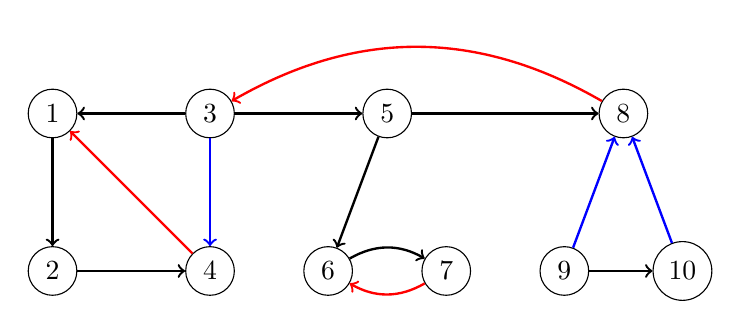
\begin{tikzpicture}[]
 \node[circle,draw=black] (1) at (0,2) {$1$};
 \node[circle,draw=black] (2) at (0,0) {$2$};
 \node[circle,draw=black] (3) at (2,2) {$3$};
 \node[circle,draw=black] (4) at (2,0) {$4$};
 \node[circle,draw=black] (5) at (4.25,2) {$5$};
 \node[circle,draw=black] (6) at (3.5,0) {$6$};
 \node[circle,draw=black] (7) at (5,0) {$7$};
 \node[circle,draw=black] (8) at (7.25,2) {$8$};
 \node[circle,draw=black] (9) at (6.5,0) {$9$};
 \node[circle,draw=black] (10) at (8,0) {$10$};

% Baumkanten
 \draw[->,line width=0.3mm] (1) edge (2);
 \draw[->,line width=0.3mm] (2) edge (4);
 \draw[->,line width=0.3mm] (3) edge (1) (3) edge (5);
 \draw[->,line width=0.3mm] (5) edge (6) (5) edge (8); 
 \draw[->,line width=0.3mm] (6) to[bend left] (7);
 \draw[->,line width=0.3mm] (9) edge (10);

% Rückwärtskanten
 \draw[->,line width=0.3mm,red] (4) edge (1);
 \draw[->,line width=0.3mm,red] (7) to[bend left] (6);
 \draw[->,line width=0.3mm,red] (8) to[bend right] (3);

% Vorwärtskanten
 \draw[->,line width=0.3mm,blue] (3) edge (4);
 \draw[->,line width=0.3mm,blue] (9) edge (8);
 \draw[->,line width=0.3mm,blue] (10) edge (8); 
	
% Querkanten (keine vorhanden..)
	
\end{tikzpicture}
\end{center} 
\end{bsp} 

\begin{bem} 
In einem ungerichteten Graphen können bei der Klassifizierung der Kanten nach Definition~\ref{def:kantenarten-tiefensuche} Mehrdeutigkeiten auftreten, da die Kanten $uv$ und $vu$ übereinstimmen.
Daher klassifizieren wir hier die Kanten in Abhängigkeit davon, ob der Algorithmus zuerst $uv$ oder zuerst $vu$ sondiert. 

Als weitere Besonderheit bei ungerichteten Graphen bemerken wir noch, dass während einer Tiefensuche weder Vorwärts- noch Querkanten auftreten:
\end{bem} 

\begin{thm}
Bei einer Tiefensuche auf einem ungerichteten Graphen $G$ ist jede Kante entweder eine Baumkante oder eine Rückwärtskante.
\end{thm}

\begin{proof}
Sei $(u,v)$ eine beliebige Kante von~$G$ und seien die Knoten so bezeichnet, dass $\cc{Grau}[u] < \cc{Grau}[v]$ gilt.
Die Tiefensuche muss daher den Knoten~$v$ entdeckt und fertig abgearbeitet haben, bevor~$u$ fertig abgearbeitet ist.
In der Zwischenzeit ist der Knoten~$u$ stets grau.
Falls die Durchmusterung die Kante zuerst in der Richtung von~$u$ nach~$v$ sondiert, so ist~$v$ bis dahin unentdeckt (also weiß) gewesen, da die Kante sonst bereits in Gegenrichtung sondiert worden wäre.
Mit anderen Worten, die Kante $(u,v)$ ist eine Baumkante.

Falls nun die Durchmusterung die Kante zuerst in der Richtung von~$v$ nach~$u$ sondiert, so ist die Kante $(u,v)$ eine Rückwärtskante, da~$u$ zu dem Zeitpunkt der Sondierung noch grau ist.
\end{proof}




\subsection{Anwendung I -- Topologisches Sortieren}

\begin{defn} 
Sei $D=(V,A)$ ein Digraph mit $n$ Knoten.
Eine \emph{topologische Sortierung} von $D$ ist eine Anordnung $v_1,\ldots,v_n$ seiner Knoten, so dass $i < j$ gilt, falls $(v_i,v_j) \in A$ eine Kante in~$D$ ist.
Das heißt, der Startknoten einer jeden Kante kommt in der Anordnung vor dem Endknoten.
\end{defn} 

\begin{bem}
Man kann die topologische Sortierung auch als horizontale Anordnung der Knoten von~$D$ auffassen, so dass jede Kante von links nach rechts zeigt.

Diese Veranschaulichung zeigt, dass es nicht möglich ist, einen Digraphen topologisch zu sortieren, wenn er einen Zyklus enthält.
Im Folgenden werden wir sehen, wie man mit einer Tiefensuche jeden \emph{azyklischen} Digraphen topologisch sortieren kann.
Als Konsequenz ergibt sich:
\end{bem} 

\begin{prop}
Ein Digraph besitzt genau dann eine topologische Sortierung, wenn er azyklisch ist.
\end{prop}

\begin{bem} 
Das topologische Sortieren kann also als Methode verstanden werden, um zu testen ob es Zyklen im Eingabegraphen gibt.
Eine andere Anwendung ist das Sequenzieren von Aufträgen (engl.~\emph{scheduling}).
Zum Beispiel hilft die topologische Sortierung zu entscheiden, in welcher Reihenfolge einzelne Teilprojekte in einem großen Programmierprojekt kompiliert werden sollten.
\end{bem} 

\begin{bem} 
Eine vollständige Tiefensuche wird zu einer Methode zum topologischen Sortieren, indem man während der Suche den jeweils nächsten abgearbeiteten Knoten notiert.
Konkret wird das gewöhnlich mittels des Verwaltens einer einfach verketteten Liste implementiert:

\begin{algorithm}[H]
\caption{$\cc{Topologisches-Sortieren}(D)$}
 \begin{algorithmic}[1]
  \STATE $L:=\cc{nil}$ $\quad$ \COMMENT{Eine leere einfach verkettete Liste anlegen}
  \STATE $\cc{Vollständige-Tiefensuche}(D)$ mit folgender Modifikation:
  \STATE $\qquad$ nach Zeile~\ref{line:schwarzfaerbung-in-tiefensuche} in $\cc{Tiefensuche}(u)$: Füge $u$ am Kopf von $L$ hinzu.
 \end{algorithmic}
\end{algorithm}
\end{bem} 

\begin{bem}
Der Algorithmus sortiert die Knoten von~$D$ also absteigend nach den Einträgen im Array $\cc{Schwarz}$.
Wir könnten also auch erst eine vollständige Tiefensuche auf~$D$ ausführen, und dann das Array $\cc{Schwarz}$ absteigend sortieren um eine topologische Sortierung zu erhalten.
Da nach unserem Wissensstand das Sortieren eines Arrays der Länge $|V|$ im schlechtesten Fall eine Laufzeit von $\Theta(|V|\log|V|)$ hat, würden wir auf diese Weise einen Algorithmus mit der Laufzeit $\Theta(|V|\log|V| + |A|)$ erhalten.
Das Aufbauen der topologisch sortierten Liste während der Tiefensuche führt zu optimaler linearer Laufzeit:
\end{bem} 

\begin{thm}
Ist ein azyklischer Digraph $D=(V,A)$ als Adjazenzliste gegeben, so benötigt der Algorithmus $\cc{Topologisches-Sortieren}(D)$ genau $\Theta(|V|+|A|)$ Zeiteinheiten.
\end{thm}

\begin{proof}
Nach Theorem~\ref{thm:laufzeit-tiefensuche} wissen wir, dass die vollständige Tiefensuche auf~$D$ die Laufzeit $\Theta(|V|+|A|)$ hat.
Die topologische Sortierung erfolgt durch das Einfügen des Knotens~$v$ an den Kopf einer einfach verketteten Liste, sobald der Zeitstempel $\cc{Schwarz}[v]$ gesetzt wird.
Ein solches Einfügen erfordert $\Theta(1)$ Zeiteinheiten.
Da jeder Knoten genau einmal in die Liste eingefügt wird, ist der gesamte zusätzliche Aufwand $\Theta(|V|)$ und wir sind fertig.
\end{proof}

\begin{bem} 
Um die Korrektheit des topologischen Sortierens über die oben beschriebene Tiefensuche zu beweisen, benutzen wir unser Wissen über die Charakterisierung der Kanten.
\end{bem} 

\begin{lem}
\label{lem:azyklisch-rueckwarts}
Ein Digraph $D=(V,A)$ ist genau dann azyklisch, wenn eine Tiefensuche auf $D$ keine Rückwärtskanten produziert.
\end{lem}

\begin{proof}
\glqq $\Longrightarrow$\grqq: Angenommen eine Tiefensuche auf~$D$ produziert eine Rückwärtskante $(u,v)$.
Dann ist $v$ ein Vorfahre von $u$ im zugehörigen Tiefensuchwald.
Somit enthält~$D$ einen Pfad von $v$ nach $u$, der zusammen mit der Kante $(u,v)$ einen Zyklus ergibt.

\glqq $\Longleftarrow$\grqq: Nehmen wir hier zum Widerspruch an, dass~$D$ einen Zyklus $Z$ enthält.
Sei~$v$ der erste Knoten, der im Zyklus $Z$ bei der Tiefensuche entdeckt wird, und sei $(u,v)$ die Kante von $Z$, die $v$ als Endknoten hat.
Zum Zeitpunkt $\cc{Grau}[v]$ bilden die Knoten in $Z$ einen Pfad, der bis auf den Knoten~$v$ nur aus weißen Knoten besteht.
Nach dem Theorem der weißen Pfade (Theorem~\ref{thm:weisse-pfade-thm}), ist dann $u$ Nachfahre von $v$ im Tiefensuchwald.
Mit anderen Worten, $(u,v)$ ist eine Rückwärtskante.
\end{proof}

\begin{thm}
Der Algorithmus $\cc{Topologisches-Sortieren}(D)$ erzeugt für jeden azyklischen Digraphen~$D=(V,A)$ eine korrekte topologische Sortierung.
\end{thm}

\begin{proof}
Wie oben diskutiert, besteht das topologische Sortieren mittels der Tiefensuche lediglich darin, einmal den Algorithmus $\cc{Vollständige-Tiefensuche}(D)$ auszuführen und dann die Knoten in absteigender Reihenfolge nach Zeitpunkten der Abarbeitung ($=$ Schwarzfärbung) auszugeben.
Wir müssen also zeigen, dass die Ungleichung $\cc{Schwarz}[v] < \cc{Schwarz}[u]$ für jede Kante $(u,v) \in A$ nach dem Abschluss der Tiefensuche gilt.

Sei dazu $(u,v) \in A$ eine beliebige Kante in~$D$.
Während $(u,v)$ sondiert wird, kann~$v$ nicht grau sein, da sonst~$v$ ein Vorfahre von~$u$ im Tiefensuchwald und damit $(u,v)$ eine Rückwärtskante wäre - im Widerspruch zur Zyklenfreiheit von~$D$ und Lemma~\ref{lem:azyklisch-rueckwarts}.
Der Knoten~$v$ ist beim Sondieren von $(u,v)$ also entweder weiß oder schwarz.
Falls~$v$ weiß ist, so wird er ein Nachfahre von~$u$ sein, und damit $\cc{Schwarz}[v] < \cc{Schwarz}[u]$ gelten.
Ist~$v$ schwarz, so ist der Knoten bereits abgearbeitet und der Zeitstempel $\cc{Schwarz}[v]$ bereits gesetzt.
Da bei der Sondierung von $(u,v)$ der Knoten~$u$ noch grau ist, wird in diesem Fall also auch $\cc{Schwarz}[v] < \cc{Schwarz}[u]$ gelten.
\end{proof}


\subsection{Anwendung II -- Starke Zusammenhangskomponenten}

\begin{defn}
Eine inklusionsmaximale Teilmenge $K \subseteq V$ der Knoten eines gegebenen Digraphen $D=(V,A)$ heißt \emph{starke Zusammenhangskomponente}, wenn es für jedes Paar von Knoten $u,v \in K$ sowohl einen $(u,v)$-Pfad als auch einen $(v,u)$-Pfad in~$D$ gibt.
Das heißt, die Knoten $u$ und $v$ sind vom jeweils anderen aus erreichbar.
\end{defn} 

\begin{bsp}
\label{bsp:starke-zusammenhangskomponenten}
Die starken Zusammenhangskomponenten des Digraphen aus Beispiel~\ref{bsp:tiefensuche} bestehen aus den Knoten gleicher Farbe in folgender Abbildung:

\hfill
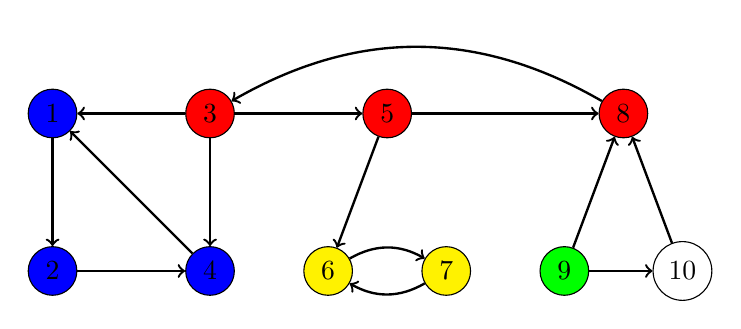
\begin{tikzpicture}[]
 \node[fill=blue,circle,draw] (1) at (0,2) {$1$};
 \node[fill=blue,circle,draw] (2) at (0,0) {$2$};
 \node[fill=red,circle,draw] (3) at (2,2) {$3$};
 \node[fill=blue,circle,draw] (4) at (2,0) {$4$};
 \node[fill=red,circle,draw] (5) at (4.25,2) {$5$};
 \node[fill=yellow,circle,draw] (6) at (3.5,0) {$6$};
 \node[fill=yellow,circle,draw] (7) at (5,0) {$7$};
 \node[fill=red,circle,draw] (8) at (7.25,2) {$8$};
 \node[fill=green,circle,draw] (9) at (6.5,0) {$9$};
 \node[circle,draw=black] (10) at (8,0) {$10$};
		
 \draw[->,line width=0.3mm] (1) edge (2);
 \draw[->,line width=0.3mm] (2) edge (4);
 \draw[->,line width=0.3mm] (3) edge (1) (3) edge (4) (3) edge (5);
 \draw[->,line width=0.3mm] (4) edge (1);
 \draw[->,line width=0.3mm] (5) edge (6) (5) edge (8); 
 \draw[->,line width=0.3mm] (6) to[bend left] (7);
 \draw[->,line width=0.3mm] (7) to[bend left] (6);
 \draw[->,line width=0.3mm] (8) to[bend right] (3);
 \draw[->,line width=0.3mm] (9) edge (8) (9) edge (10);
 \draw[->,line width=0.3mm] (10) edge (8); 
\end{tikzpicture}
\hfill\,
\end{bsp}

\begin{bem}
Als weitere wichtige Anwendung der Tiefensuche zeigen wir hier, wie man mit ihrer Hilfe einen Digraphen in dessen starken Zusammenhangskomponenten zerlegen kann, das heißt, wir suchen eine Partition $V = K_1 \cup K_2 \cup \ldots \cup K_r$ der Knotenmenge von~$D$, so dass jede Teilmenge $K_i \subseteq V$ eine starke Zusammenhangskomponente ist.
Eine solche Zerlegung liegt vielen Algorithmen auf Digraphen zugrunde, da sie einen Ansatz mittels des Schemas Teile-und-Beherrsche erlaubt:
Nach der erfolgten Zerlegung des Digraphen arbeitet der jeweilige Algorithmus auf den einzelnen Komponenten separat und vereinigt dann die Lösungen entsprechend der Verbindungsstruktur der Komponenten untereinander.

Der Algorithmus, den wir hier untersuchen wollen, basiert darauf eine Tiefensuche auf dem gegebenen Digraphen $D=(V,A)$ und danach eine weitere auf seinem \emph{transponierten Graphen} $D^T = (V,A^T)$ zu machen, dessen Kantenmenge durch $A^T = \{(u,v) \in V \times V : (v,u) \in A\}$ definiert ist.
Wir erhalten also $D^T$ aus $D$ indem wir die Orientierung aller Kanten von $D$ umdrehen.

Ein Knoten $v$ ist in $D$ genau dann von einem anderen Knoten $u$ aus erreichbar, wenn~$u$ in $D^T$ von $v$ aus erreichbar ist.
Es gilt weiterhin die folgende wichtige Eigenschaft:
\end{bem} 

\begin{prop}
\label{beob:d-vs-dt}
Der zu einem Digraphen $D=(V,A)$ transponierte Graph $D^T$ hat dieselben starken Zusammenhangskomponenten wie~$D$.
\end{prop}

\begin{bem} 
Der konkrete Algorithmus zum Bestimmen der starken Zusammenhangskomponenten ist im folgenden Pseudocode angegeben.
Beachten Sie die Modifikation der Reihenfolge, in der die Knoten bei der zweiten Tiefensuche durchlaufen werden.

\begin{algorithm}[H]
\caption{$\cc{Starke-Zusammenhangskomponenten}(D)$}
 \begin{algorithmic}[1]
  \STATE\label{line:szhk0} $\cc{Vollständige-Tiefensuche}(D)$
  \STATE berechne $D^T$
  \STATE\label{line:szhk1} $\cc{Vollständige-Tiefensuche}(D^T)$ mit folgender Modifikation:
  \STATE\label{line:szhk2} $\qquad$ Durchlaufe die Hauptschleife (Zeilen~\ref{line:tiefensuche-hauptschleife-start}--\ref{line:tiefensuche-hauptschleife-ende}) der Tiefensuche auf $D^T$ in absteigender Reihenfolge des Arrays $\cc{Schwarz}$ von~$D$.
  \STATE gib die Knoten eines jeden Baumes im Tiefensuchwald $(D^T)_\pi$ als starke Zusammenhangskomponenten aus
 \end{algorithmic}
\end{algorithm}
\end{bem} 

\begin{thm}
\label{thm:starke-zshgk-laufzeit}
Ist ein Digraph $D=(V,A)$ als Adjazenzliste gegeben, so hat der Algorithmus $\cc{Starke-Zusammenhangskomponenten}(D)$ lineare Laufzeit, das heißt, er benötigt $\Theta(|V|+|A|)$ Zeiteinheiten.
\end{thm}

\begin{proof}
Die Tiefensuche in Zeile~\ref{line:szhk0} hat nach Theorem~\ref{thm:laufzeit-tiefensuche} lineare Laufzeit.
Die Berechnung des transponierten Graphen~$D^T$ kann auch in linearer Laufzeit geschehen, da~$D$ als Adjazenzliste gegeben ist (siehe Übungsblatt 7, Aufgabe (3)).
Die modifizizerte Tiefensuche auf~$D^T$ in den Zeilen~\ref{line:szhk1}-\ref{line:szhk2} läuft wieder in Zeit $\Theta(|V|+|A|)$.
Ebenso ist die Ausgabe der Bäume im Tiefensuchwald $(D^T)_\pi$ in linearer Laufzeit möglich.
\end{proof}

\begin{bem}
Die Idee hinter dem Algorithmus $\cc{Starke-Zusammenhangskomponenten}(D)$ beruht auf dem Konzept des \emph{Komponentengraphen} $D^K=(V^K,A^K)$ von $D=(V,A)$, der wie folgt definiert ist.
Seien $K_1,\ldots,K_r$ die starken Zusammenhangskomponenten von~$D$.
Dann setzen wir $V^K:=\{v_1,\ldots,v_r\}$, also je ein Knoten~$v_i$ für je eine starke Zusammenhangskomponente~$K_i$.
Es gibt eine Kante $(v_i,v_j) \in A^K$ genau dann, wenn es ein $u \in K_i$ und ein $w \in K_j$ gibt, so dass $(u,w) \in A$ eine Kante in~$D$ ist.
Der Komponentengraph~$D^K$ ensteht also aus~$D$ indem wir alle Kanten kontrahieren, deren Start- und Endknoten zur selben starken Zusammenhangskomponente gehören.
\end{bem}

\begin{bsp}
\label{bsp:komponentengraph}
Der Komponentengraph des Digraphen aus Beispiel~\ref{bsp:starke-zusammenhangskomponenten} in derselben Farbkodierung:

\hfill
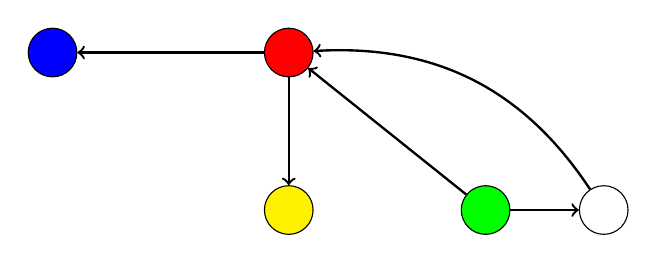
\begin{tikzpicture}[]
 \node[fill=blue,circle,draw] (1) at (1,2) {$\phantom{1}$};
% \node[fill=blue,circle,draw] (2) at (0,0) {$2$};
% \node[fill=red,circle,draw] (3) at (2,2) {$3$};
% \node[fill=blue,circle,draw] (4) at (2,0) {$4$};
 \node[fill=red,circle,draw] (5) at (4,2) {$\phantom{5}$};
 \node[fill=yellow,circle,draw] (6) at (4,0) {$\phantom{6}$};
% \node[fill=yellow,circle,draw] (7) at (5,0) {$7$};
% \node[fill=red,circle,draw] (8) at (7.25,2) {$8$};
 \node[fill=green,circle,draw] (9) at (6.5,0) {$\phantom{9}$};
 \node[circle,draw=black] (10) at (8,0) {$\phantom{0}$};
		
 \draw[->,line width=0.3mm] (5) edge (6) (5) edge (1); 
 \draw[->,line width=0.3mm] (9) edge (5) (9) edge (10);
 \draw[->,line width=0.3mm] (10) to[bend right] (5); 
\end{tikzpicture}
\hfill\,
\end{bsp}

\begin{bem}
Die wesentliche Eigenschaft des Komponentengraphen ist, dass er einen azyklischen Digraphen darstellt:
\end{bem} 

\begin{lem}
\label{lem:komponentengraph-azyklisch}
Sei $D=(V,A)$ ein Digraph und seien $K,K'$ zwei verschiedene starke Zusammenhangskomponenten von~$D$.
Seien weiterhin $u,v \in K$ und $u',v' \in K'$ Knoten der jeweiligen Komponente.
Falls $D$ einen $(u,u')$-Pfad enthält, so kann er nicht gleichzeitig auch einen $(v',v)$-Pfad enthalten.
\end{lem}

\begin{proof}
Angenommen, $D$ würde neben einem $(u,u')$-Pfad auch einen $(v',v)$-Pfad enthalten.
Da $K$ und $K'$ starke Zusammenhangskomponenten sind, könnten wir den $(u,u')$-Pfad zu einem $(u,v')$-Pfad und ebenso den $(v',v)$-Pfad zu einem $(v',u)$-Pfad erweitern.
Demnach wären die Knoten~$u$ und~$v'$ vom jeweils anderen aus erreichbar, was der Annahme widerspricht, dass $K$ und $K'$ verschieden sind.
\end{proof}

\begin{bem}
Für den Korrektheitsbeweis des angegebenen Algorithmus benötigen wir etwas mehr Verständnis der Beziehungen zwischen den während der Laufzeit erzeugten Zeitstempeln.
Wenn wir nachfolgend von Zeitpunkten der Entdeckung und Abarbeitung sprechen, dann beziehen wir uns stets auf die entsprechenden Zeitstempel der ersten Tiefensuche in Zeile~\ref{line:szhk0} von $\cc{Starke-Zusammenhangskomponenten}(D)$.

Für die Formulierung der Aussage erweitern wir zunächst die Begriffe der Entde\-ckungs- und Abarbeitungszeitpunkte von einzelnen Knoten auf Teilmengen von Knoten:
Für $U \subseteq V$ seien dazu
\[
\cc{Grau}(U) := \min_{u \in U} \cc{Grau}[u] \quad \text{ und } \quad\cc{Schwarz}(U) := \max_{u \in U} \cc{Schwarz}[u]
\]
der früheste Entdeckungszeitpunkt beziehungsweise der späteste Abarbeitungszeitpunkt eines Knotens aus~$U$.
\end{bem}

\begin{lem}
\label{lem:komponenten-zeitpunkte}
Sei $D=(V,A)$ ein Digraph und seien $K,K'$ zwei verschiedene starke Zusammenhangskomponenten von~$D$.
\begin{enumi}
 \item\label{lem:komponenten-zeitpunkte:primal} Falls eine Kante $(u,v) \in A$ mit $u \in K$ und $v \in K'$ existiert, so gilt
 \[
 \cc{Schwarz}(K) > \cc{Schwarz}(K').
 \]
 
 \item\label{lem:komponenten-zeitpunkte:transponiert} Falls eine Kante $(u,v) \in A^T$ mit $u \in K$ und $v \in K'$ existiert, so gilt
 \[
 \cc{Schwarz}(K) < \cc{Schwarz}(K').
 \]
\end{enumi}
\end{lem}

\begin{proof}
i): Wir unterscheiden Fälle danach welche der beiden starken Zusammenhangskomponenten zuerst entdeckt wird.

Sei zuerst angenommen, dass $\cc{Grau}(K) < \cc{Grau}(K')$ gilt und sei~$x$ der erste entdeckte Knoten in~$K$.
Zum Zeitpunkt $\cc{Grau}[x]$ sind alle anderen Knoten in~$K$ und alle Knoten in~$K'$ weiß.
In diesem Moment enthält~$D$ also Pfade von~$x$ zu jedem anderen Knoten in~$K$, die, bis auf~$x$ selbst, nur aus weißen Knoten bestehen.
Die Existenz der Kante $(u,v)$ von der Komponente~$K$ in die Komponente~$K'$ impliziert damit, dass ebenso Pfade von~$x$ zu jedem Knoten in~$K'$ bestehen, die, bis auf~$x$ selbst, nur aus weißen Knoten bestehen.
Nach dem Theorem~\ref{thm:weisse-pfade-thm} der weißen Pfade sind also alle Knoten in $K \cup K'$ Nachfahren von~$x$ im Tiefensuchwald und nach Korollar~\ref{cor:nachfahre-tiefenwald} erhalten wir $\cc{Schwarz}(K) = \cc{Schwarz}[x] > \cc{Schwarz}(K')$.

Sei nun angenommen, dass $\cc{Grau}(K) > \cc{Grau}(K')$ gilt und sei~$y$ der erste entdeckte Knoten in~$K'$.
Analog zu oben sind zum Zeitpunkt $\cc{Grau}[y]$ alle Knoten in~$K'$ mit einem Pfad von~$y$ aus erreichbar, der, bis auf~$y$ selbst, nur aus weißen Knoten besteht.
Wegen Theorem~\ref{thm:weisse-pfade-thm} sind damit alle Knoten aus~$K'$ Nachfahren von~$y$ im Tiefensuchwald und mit Korollar~\ref{cor:nachfahre-tiefenwald} gilt $\cc{Schwarz}[y] = \cc{Schwarz}(K')$.
Nach Annahme sind zum Zeitpunkt $\cc{Grau}[y]$ alle Knoten in~$K$ weiß.
Da die Kante $(u,v)$ von~$K$ nach~$K'$ existiert, folgt aus Lemma~\ref{lem:komponentengraph-azyklisch}, dass es keinen Pfad von einem Knoten in~$K'$ zu einem Knoten in~$K$ geben kann.
Da damit kein Knoten in~$K$ von~$y$ aus erreichbar ist, ist die ganze Komponente~$K$ zum Zeitpunkt $\cc{Schwarz}[y]$ noch immer weiß.
Als Konsequenz erhalten wir $\cc{Schwarz}[w] > \cc{Schwarz}[y]$, für jeden Knoten $w \in K$, und damit $\cc{Schwarz}(K) > \cc{Schwarz}(K')$.

ii): Nach Definition von $A^T$ ist $(v,u)$ Kante von~$D$.
Da nach Beobachtung~\ref{beob:d-vs-dt} die Teilmengen~$K$ und $K'$ starke Zusammenhangskomponenten von~$D^T$ sind, können wir Teil~i) anwenden und erhalten $\cc{Schwarz}(K) < \cc{Schwarz}(K')$.
\end{proof}

\begin{bem} 
In Worten ausgedrückt besagt das vorige Lemma, dass jede Kante von~$D$ (bzw.~$D^T$), die zwei verschiedene starke Zusammenhangskomponenten verbindet, von der Komponente mit dem späteren (bzw.~früheren) Abarbeitungszeitpunkt ausgeht.

Auf der Grundlage dieser Beobachtung können wir nun die Grundidee des Korrektheitsbeweises erläutern:
Die Tiefenssuche auf~$D^T$ startet in der starken Zusammenhangskomponente~$K_1$, die den zuletzt abgearbeiteten Knoten~$u_1$ der Tiefensuche auf~$D$ enthält.
Der transponierte Graph $D^T$ enthält nach Lemma~\ref{lem:komponenten-zeitpunkte}~\ref{lem:komponenten-zeitpunkte:transponiert} keine Kanten, die von~$K_1$ zu einer anderen starken Zusammenhangskomponente verlaufen.
Daher werden bei der Tiefensuche die von~$u_1$ aus startet genau die Knoten aus der Komponente~$K_1$ besucht.
Der Algorithmus wählt danach den Knoten~$u_2$ außerhalb der Komponente~$K_1$, der als letztes unter den verbleibenden Knoten bei der Tiefensuche auf~$D$ abgearbeitet wurde und besucht wie zuvor, alle Knoten der starken Zusammenhangskomponente~$K_2$, die~$u_2$ enthält.
Dies geht iterativ weiter bis alle Tiefensuchbäume erstellt sind, und wir sehen, dass diese den starken Zusammenhangskomponenten entsprechen.
\end{bem} 

\begin{thm}
$\cc{Starke-Zusammenhangskomponenten}(D)$ bestimmt die starken Zusammenhangskomponenten eines Digraphen~$D=(V,A)$ korrekt.
\end{thm}

\begin{proof}
Wir argumentieren über vollständige Induktion nach der Anzahl der Tiefensuchbäume, die bei der Tiefensuche auf $D^T$ in den Zeilen~\ref{line:szhk1}-\ref{line:szhk2} des Algorithmus $\cc{Starke-Zusammenhangskomponenten}(D)$ gefunden werden und zeigen, dass jeder solche Baum eine starke Zusammenhangskomponente bildet.
Die konkrete Aussage, die wir per Induktion beweisen, ist: \glqq Die ersten $k$ Tiefensuchbäume, die in den Zeilen~\ref{line:szhk1}-\ref{line:szhk2} erzeugt werden, sind starke Zusammenhangskomponenten von~$D$.\grqq

Der Induktionsanfang ist mit $k=0$ klar.
Für den Induktionsschritt, sei $B \subseteq V$ der $(k+1)$-te erzeugte Baum bei der Tiefensuche auf~$D^T$.
Sei weiterhin $u \in B$ die Wurzel dieses Baumes und $K \subseteq V$ die starke Zusammenhangskomponente, die~$u$ enthält.
Für jede starke Zusammenhangskomponente $K' \neq K$, die bereits besucht wurde, gilt $\cc{Schwarz}[u] = \cc{Schwarz}(K) > \cc{Schwarz}(K')$, wegen der Reihenfolge in der die Knoten in Zeile~\ref{line:szhk2} durchlaufen werden.
Wegen der Induktionsannahme sind zum Zeitpunkt zu dem die Suche den Knoten~$u$ besucht, alle anderen Knoten von~$K$ weiß.
Nach dem Theorem~\ref{thm:weisse-pfade-thm} der weißen Pfade sind daher alle anderen Knoten in~$K$ Nachfahren von~$u$ in dessen Tiefensuchbaum.

Weiterhin müssen nach Induktionsannahme und Lemma~\ref{lem:komponenten-zeitpunkte}~\ref{lem:komponenten-zeitpunkte:transponiert} alle Kanten von~$D^T$, die aus $K$ herausführen, zu starken Zusammenhangskomponenten verlaufen, die bereits entdeckt wurden.
Damit wird kein Knoten außerhalb von~$K$ ein Nachfahre von~$u$ bei der Tiefensuche auf~$D^T$.
Das heißt, dass die Knoten des Tiefensuchbaumes von~$D^T$, der von~$u$ ausgeht, eine starke Zusammenhangskomponente bilden, und der Induktionsschritt ist gezeigt.
\end{proof}
